%Capítulo 3

Este trabajo busca cumplir con la propuesta original realizada por Eduintegral, al crear una aplicación móvil la cual búsca crear, manetener y fortalecer el vinculo entre padres de familia y maestros. \\ Más aparte esta propuesta búsca ampliar la forma en la que se almacenan los datos, cumplir con la parte de administración de la aplicación y más aparte considerar un flujo seguro en el almacenamiento de los datos generados por la aplicación. \\ El objetivo primordial de Eduintegral sigue siendo el asegurar un buen desempeño del alumno basandonos en la mejora de la comunicación entre el maestro y los padres de familia, los cuales al tener una buena comunicación pódran detectar y solucionar problematicas en el desempeño de los alumnos.

\section{Modelo conceptual}
    
    El modelo conceptual del proyecto de mejora sobre Eduintegral se basa a partir de las caracteristicas definidas en la sección previa (ver sección 2.3). \\ El siguiente diagrama conceptual muestra de manera teórica como se desea que se comporte el sistema de manera generalizada (ver figura 3.1).
    
    \begin{figure}[H]
        \centering
        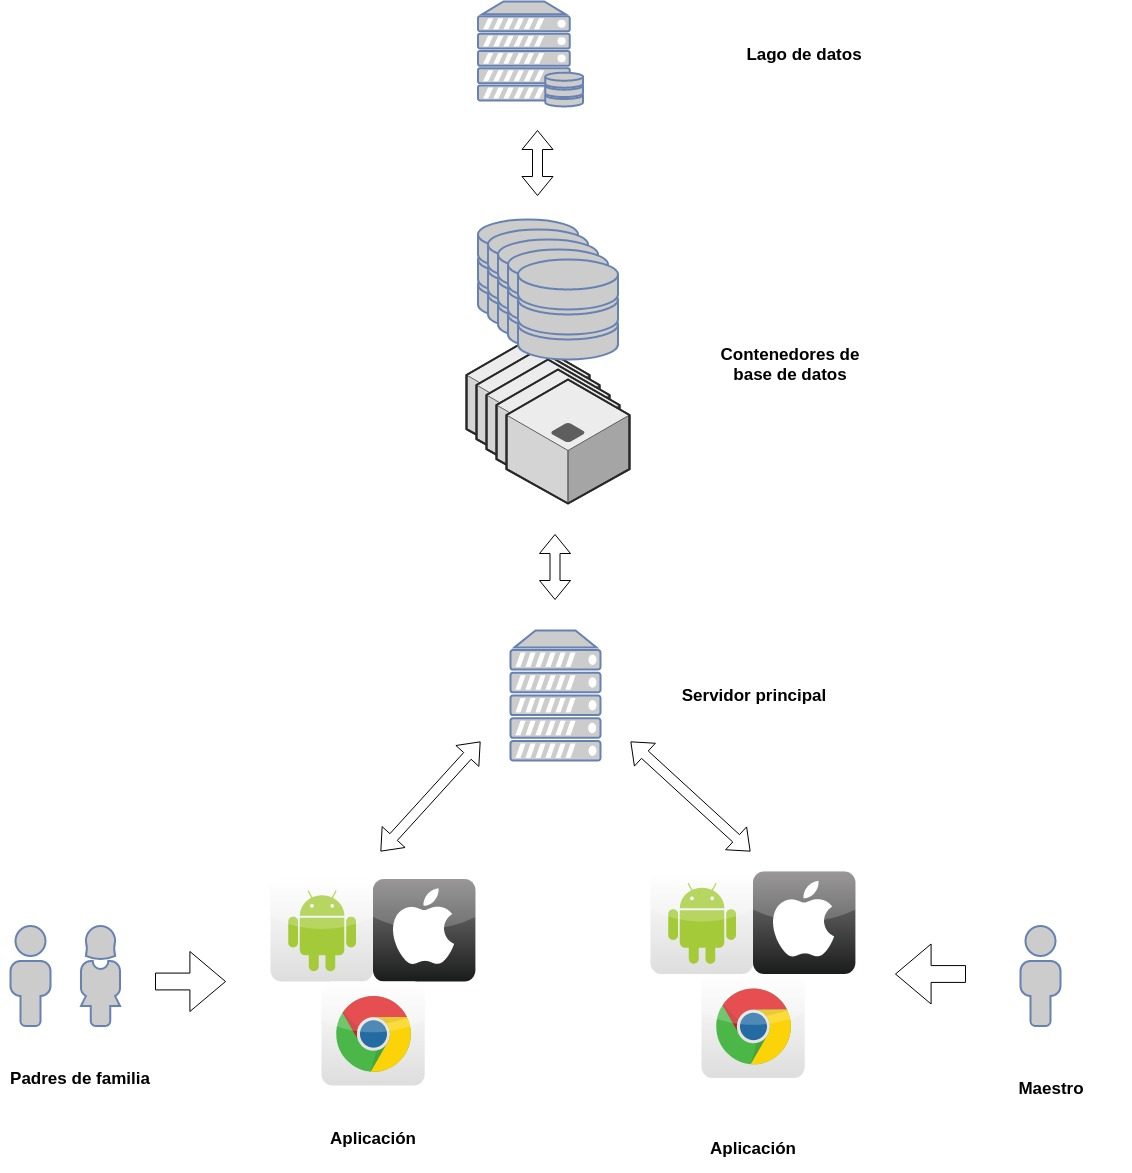
\includegraphics[scale=0.3]{imagenes/arquitectura_propuesta.jpg}
        \caption{Diagrama modelo conceptual}
        \label{fig:diagramamodeloconceptual}
    \end{figure}
    
    \begin{itemize}
    
        \item \textbf{Maestro:} Captura las calificiones de alumnos, registra la asistencia y ausencias de los alumnos, manda reportes a los padres de familia si los alumnos incurren en faltas
        
        \item \textbf{Padres de familia:} Consultan las calificaciones, ausencias y asistencias de sus hijos, recibe notificaciones por parte de los maestros
        
        \item \textbf{Aplicación:} Aplicación móvil y aplicación web capaz de servir como medio de consulta y captura de las calificaciones, asistencias y ausencias, tambien es capaz de manejar el envio de notificaciones de maestros a padres de familia
        
        \item \textbf{Servidor principal:} Es el servidor físico el cual albergara los contenedores de bases de datos, en el tambien se almacerá de momento el lago de datos
        
        \item \textbf{Contenedores de base de datos:} Estructura propuesta de manejo de contenedores con bases de datos
        
        \item \textbf{Lago de datos:} Lago de datos que almacenara todos los datos generados por el sistema
        
    \end{itemize}
    
    
\section{Base de datos}
    
    La base de datos es una de las partes principales de la arquitectura de este proyecto dado que esta tendra la estructura requeridad para almacenar todos los datos generados por la aplicación. \\ Se pretende cambiar completamente el diseño de la base de datos para que esta puede manejar mayores cantidades de datos y a su vez prepararla para soportar de manera eficiente la cantidad de consultas que se espera por todos los maestros y padres de familia de las escuelas. \\ Las caracteristicas principales encontradas para establecer esta propuesta sobre el diseño de la base de datos son:
    
    \begin{itemize}
        \item Se requiere tener registro de todos los usuarios capaces de acceder a la aplicación, un dato importante a considerar es que se tienen que diferenciar maestros de padres de familia
        
        \item Toda la información personal que rodea al alumno dentro del ámbito escolar, dicese de datos como el nombre, grado y grupo, ciclo escolar que esta cursando
        
        \item Se considera importante el tener registro sobre las asistencias y ausencias de los alumnos, teniendo en cuenta que estas se pueden dar por materias
        
        \item Es necesario conocer cuales son las materias impartidas en una especifica escuela
        
        \item Para la comunicación del padre de familia y el maestro se concentraran los reportes y los tipos de reportes que se generen
        
        \item Las calificaciones del alumno se mantendran registradas dado que es un indicador importante sobre el demsempeño estudiantil
        
        \item Los datos de maestros y padres de familia serán ligados a los datos de los alumnos 
        
        \item Se considera relevante almacenar la información pertinente de las escuelas en las que se encuentran laborando los maestros y por ende estudiando los alumnos
        
    \end{itemize}
    
    El siguiente diagrama (ver figura 3.2) muestra el diseño original de la primer base de datos propuesta para Eduintegral \cite{eduintegral}, más el diseño extendido de la base de datos propuesta en este trabajo, en la cual se consideran otras entidades adicionales que se cree ayudarán a tener la mayor cantidad de datos relevantes.
    
    \begin{figure}[H]
        \centering
        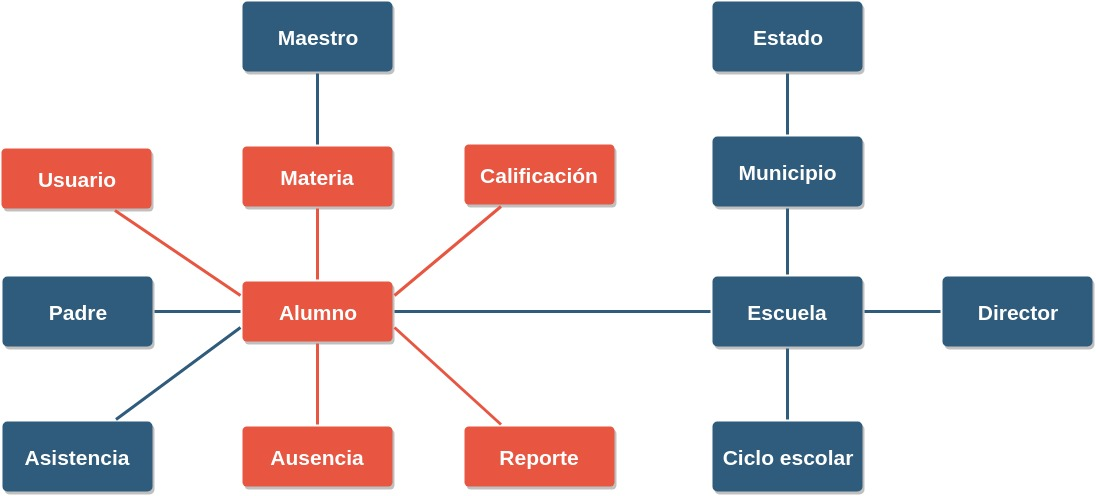
\includegraphics[scale=0.4]{Propuesta_Plantilla_Tesis_LaTeX_UAG/imagenes/base_de_datos_2.jpg}
        \caption{Diagrama de base de datos}
        \label{fig:diagramabasededatos}
    \end{figure}
    
    \begin{itemize}
    
        \item \textbf{Diagrama color rojo:} Diseño de base de datos original generado para el desarrollo de Eduintegral \cite{eduintegral}
        
        \item \textbf{Diagrama color verde:} Diseño de base de datos que contiene el diseño original propuesto más entidades que expanden la capacidad de almacenamiento de datos
        
    \end{itemize}